\documentclass[11pt,a4paper]{article}

\usepackage[T1]{fontenc}
\usepackage[utf8]{inputenc}
\usepackage[main=french,provide=*]{babel}
\usepackage{lmodern}
\usepackage[a4paper,margin=2.2cm]{geometry}
\usepackage{graphicx}
\usepackage{booktabs}
\usepackage{array}
\usepackage{tabularx}
\usepackage{float}
\usepackage{xcolor}
\usepackage{hyperref}

\hypersetup{
  colorlinks=true,
  linkcolor=black,
  urlcolor=blue,
  pdftitle={Rapport Desk - Moteur d'Analyse Technique et Dashboard},
  pdfauthor={Taha Dazine}
}

\setlength{\parindent}{0pt}
\setlength{\parskip}{0.55em}
\renewcommand{\arraystretch}{1.18}

\begin{document}
\pagenumbering{gobble}

\begin{titlepage}
\centering
\vspace*{2.5cm}

{\Huge \bfseries Moteur d'Analyse Technique\\[0.2cm] et Dashboard de Signaux\par}
\vspace{0.9cm}
{\Large Support de présentation à destination du desk\par}

\vspace{1.6cm}
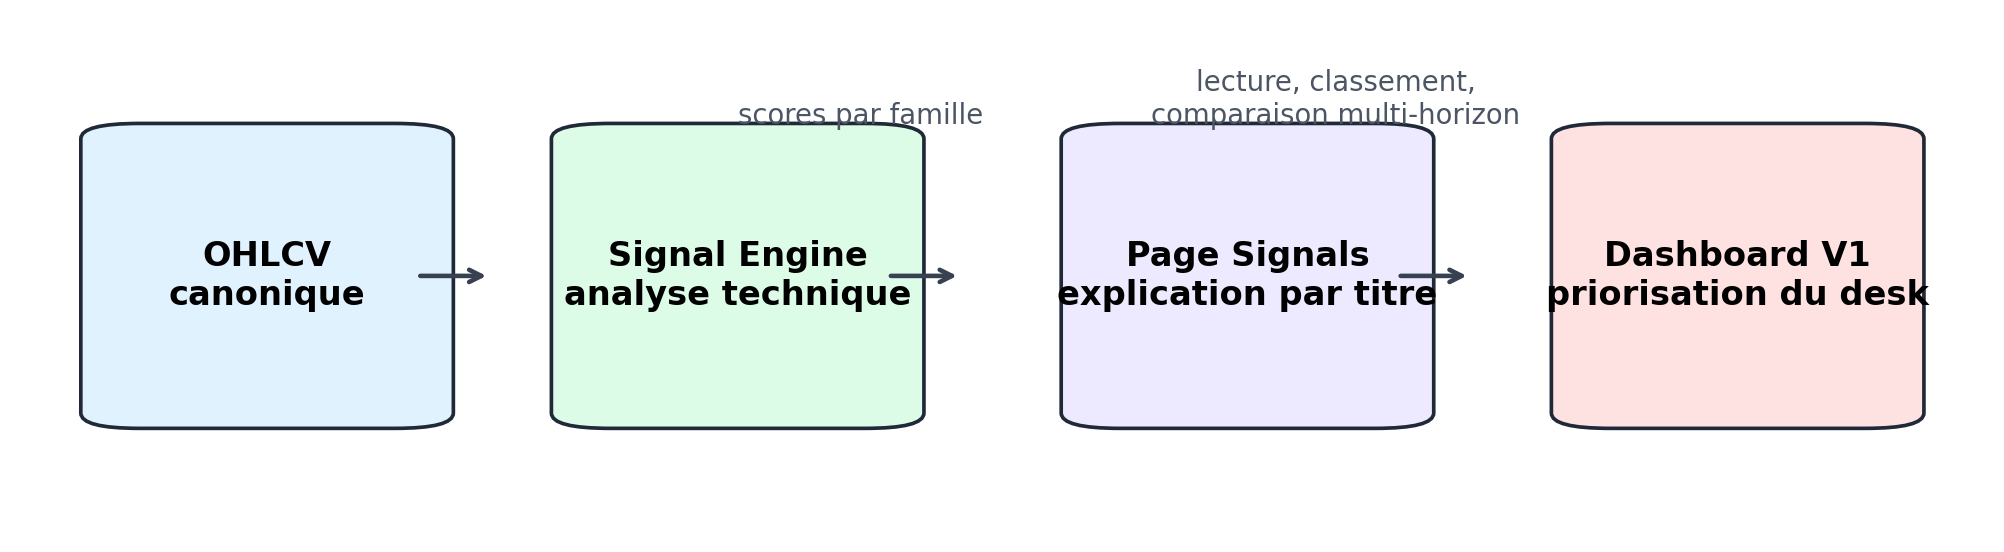
\includegraphics[width=0.9\textwidth]{figures/desk_signal_report/product_flow.png}

\vspace{1.4cm}
\begin{minipage}{0.9\textwidth}
\small
Ce document présente la brique d'analyse technique développée dans le cadre d'un stage, avec un objectif simple : fournir au desk une lecture des signaux plus structurée, plus homogène et plus justifiable. Le produit n'est pas un moteur de décision autonome. Il agit comme un outil d'aide à l'analyse et à la priorisation.
\end{minipage}

\vfill
{\large Avril 2026\par}
\end{titlepage}

\clearpage
\pagenumbering{arabic}

\section*{1. Contexte et problématique métier}

Sur un desk actions, la lecture technique doit être rapide, comparable et explicable. En pratique, ces trois exigences sont rarement réunies. Une lecture trop manuelle devient hétérogène d'un titre à l'autre. Une lecture trop simplifiée masque la provenance réelle du signal. Une lecture trop dépendante d'un seul paramètre historique expose à des conclusions fragiles.

Le produit présenté répond à ce besoin concret : \textbf{industrialiser la lecture technique d'un univers actions sans transformer l'analyse en boîte noire}. L'objectif n'est pas de remplacer le jugement du desk, mais de fournir un cadre robuste pour :

\begin{itemize}
\item repérer rapidement les titres prioritaires ;
\item distinguer le court, le moyen et le long terme ;
\item remonter du score global vers une explication intelligible ;
\item limiter l'influence de signaux fragiles ou redondants.
\end{itemize}

\begin{figure}[H]
\centering
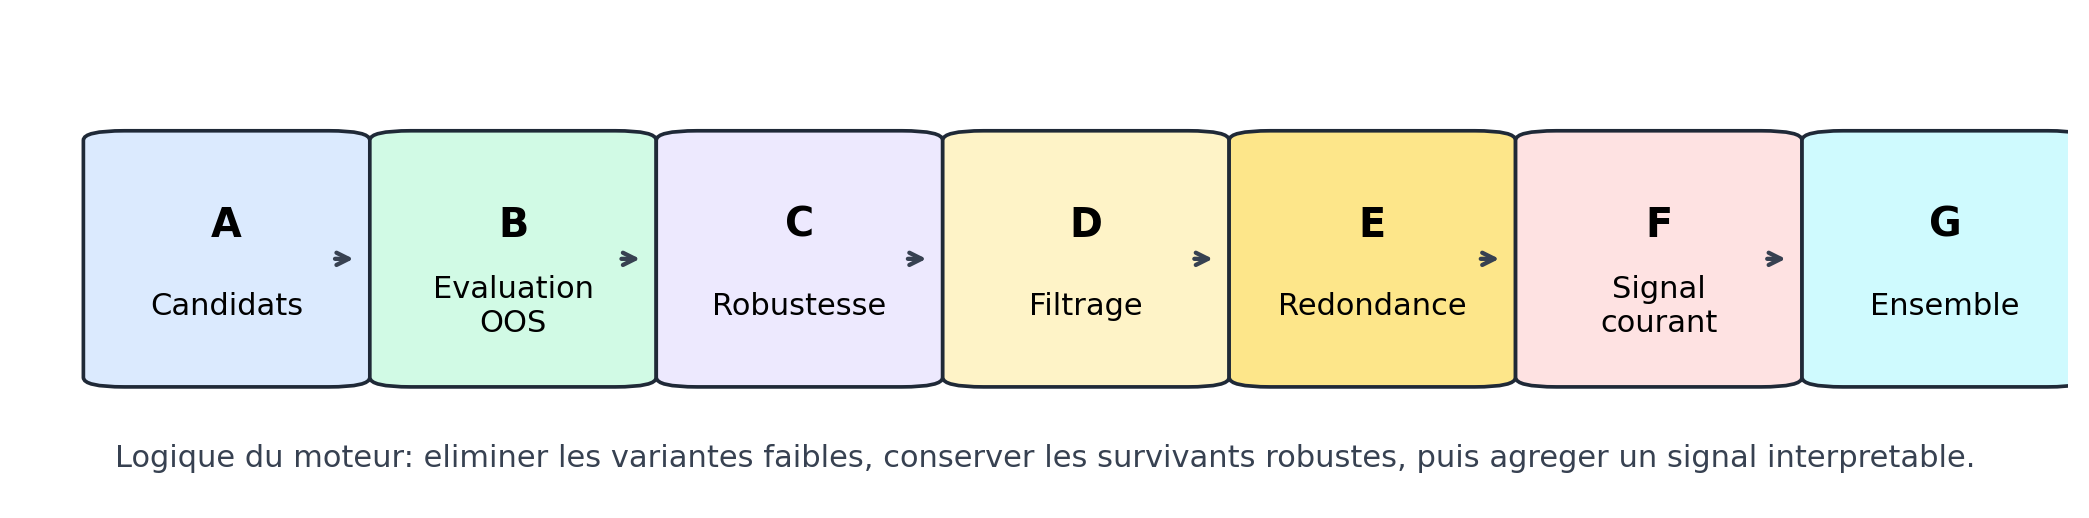
\includegraphics[width=\textwidth]{figures/desk_signal_report/pipeline_ag.png}
\caption{Pipeline A-G du moteur de signaux.}
\end{figure}

\section*{2. Présentation de la solution}

Le socle livré repose sur trois éléments complémentaires :

\begin{itemize}
\item un \textbf{Signal Engine} qui transforme les données OHLCV en scores techniques interprétables ;
\item la page \textbf{Signals}, qui permet d'analyser un titre en détail ;
\item le \textbf{dashboard V1}, qui restitue une vue de synthèse exploitable par le desk.
\end{itemize}

La logique fonctionnelle est la suivante : \textbf{OHLCV canonique \textrightarrow{} Signal Engine \textrightarrow{} page Signals \textrightarrow{} Dashboard V1}.

Le périmètre publié et mis en avant pour la présentation repose sur \textbf{quatre familles cœur} :

\begin{itemize}
\item \textbf{SMA} pour la tendance ;
\item \textbf{MACD} pour le momentum ;
\item \textbf{RSI} pour l'oscillation ;
\item \textbf{OBV} pour la lecture du volume.
\end{itemize}

Le moteur ne cherche pas à retenir le ``meilleur'' paramètre historique. Il applique une logique de recherche disciplinée : génération de variantes, évaluation \textit{out-of-sample}, scoring de robustesse, filtrage, réduction de redondance, puis agrégation finale.

\begin{table}[H]
\centering
\small
\begin{tabularx}{\textwidth}{>{\bfseries}p{2.2cm}X}
\toprule
Sortie & Utilité métier \\
\midrule
Score global par titre & Prioriser rapidement l'univers couvert \\
Lecture par famille & Comprendre l'origine du signal technique \\
Variantes retenues & Justifier la lecture au-delà d'une simple étiquette \\
Vue secteurs / indice & Situer les signaux dans un cadre transversal \\
Lecture par horizon & Distinguer le tactique du plus structurel \\
Niveaux techniques & Ajouter des repères immédiatement exploitables \\
\bottomrule
\end{tabularx}
\caption{Sorties concrètes produites par l'application.}
\end{table}

\section*{3. Fonctionnement global}

Le pipeline A-G peut être lu de façon très simple.

\textbf{A. Génération des candidats} : le moteur explore plusieurs variantes d'indicateurs plutôt que de parier sur un seul réglage.

\textbf{B. Évaluation hors échantillon} : chaque variante est testée sur des fenêtres successives selon une logique \textit{walk-forward}. Le but est de réduire le risque d'illusion historique.

\textbf{C. Scoring de robustesse} : le système mesure la fiabilité des variantes à partir de la performance ajustée, de la stabilité dans le temps, de la régularité et du drawdown.

\textbf{D-E. Filtrage et réduction de redondance} : les variantes trop faibles ou trop proches les unes des autres sont éliminées.

\textbf{F-G. Signal courant et ensemble final} : les survivants produisent un signal actuel, puis sont agrégés dans un score final interprétable.

Cette logique a une conséquence utile pour le desk : le système produit un signal \textbf{à la fois synthétique et traçable}. La page \textbf{Signals} sert à expliquer. Le \textbf{dashboard} sert à arbitrer l'attention.

\begin{figure}[H]
\centering
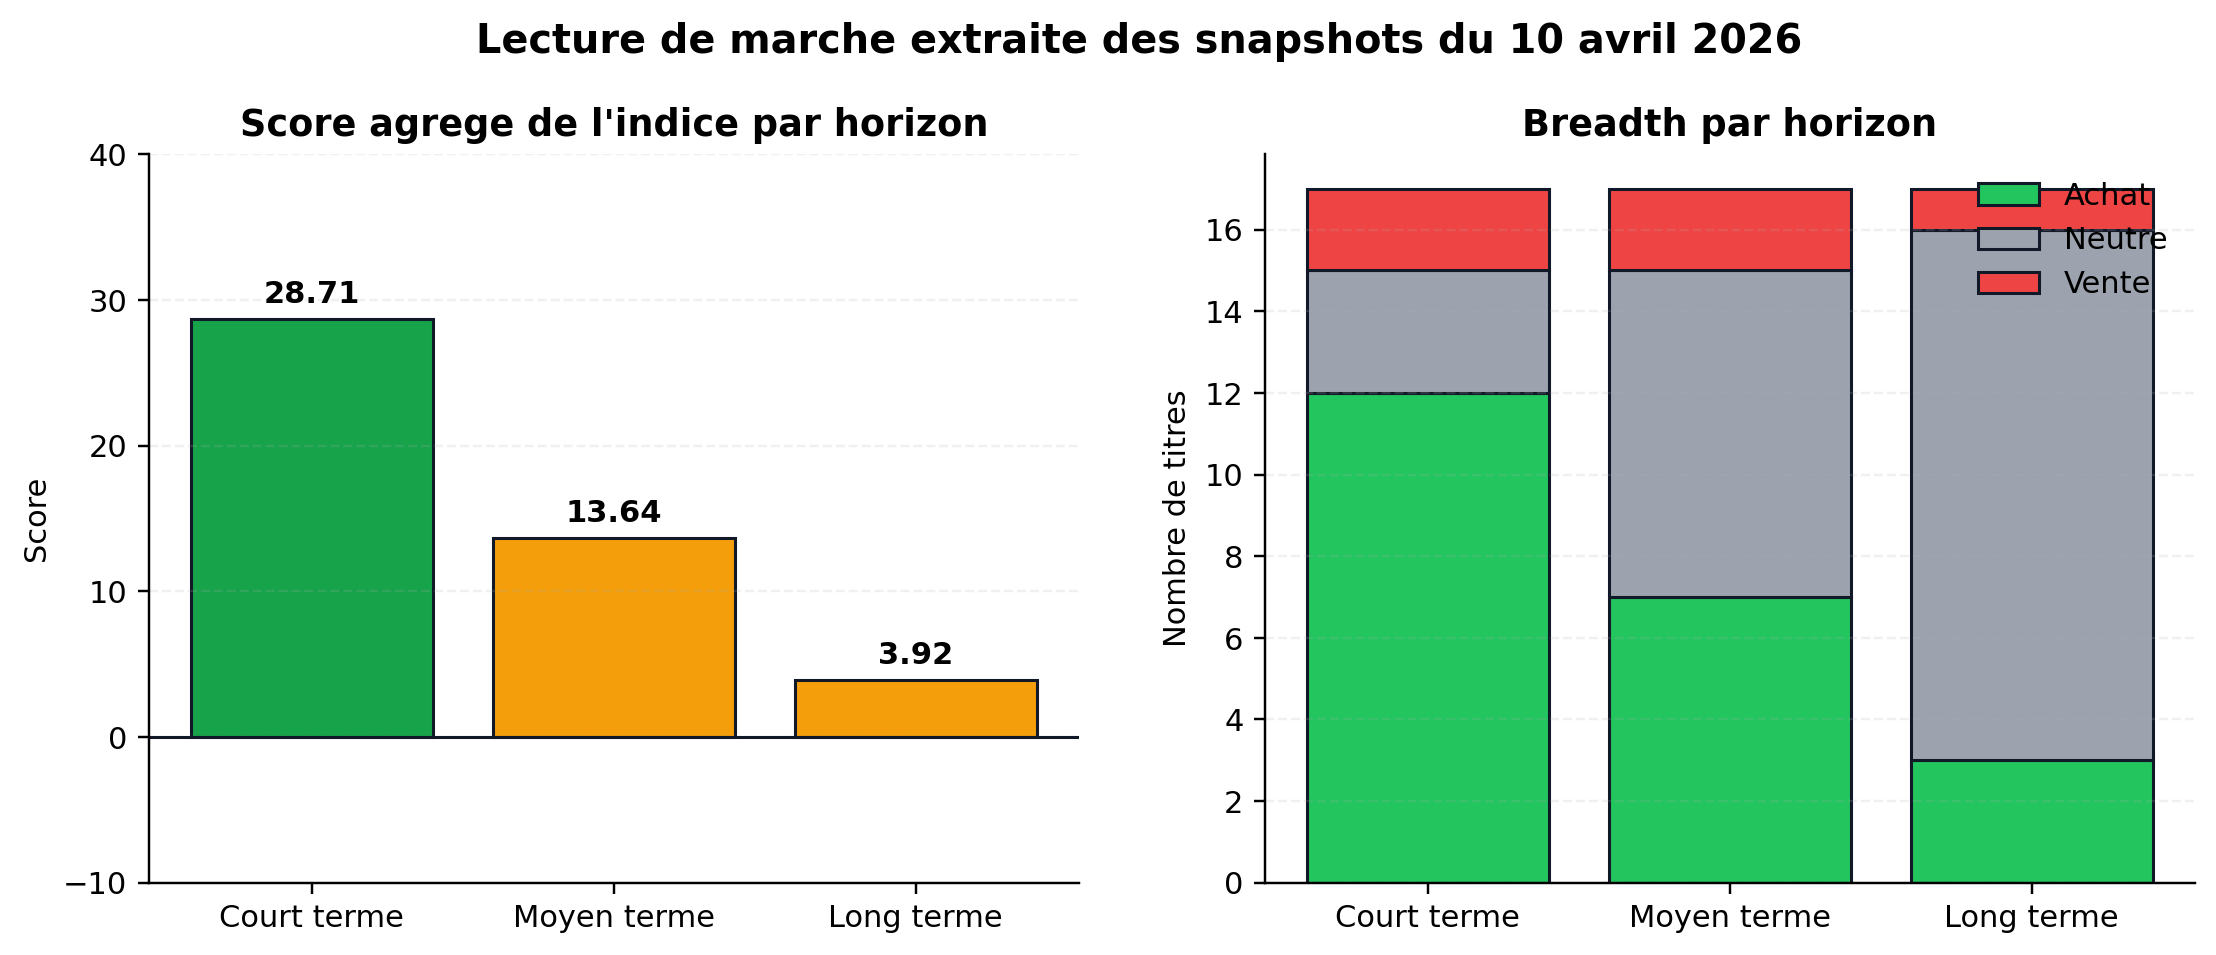
\includegraphics[width=\textwidth]{figures/desk_signal_report/market_overview.png}
\caption{Lecture de marché par horizon, extraite des snapshots du 10 avril 2026.}
\end{figure}

\section*{4. Résultats illustratifs}

Les snapshots du \textbf{10 avril 2026} montrent une lecture différenciée selon l'horizon :

\begin{itemize}
\item \textbf{court terme} : score indice de \textbf{+28,71}, soit une lecture \textbf{Achat} ;
\item \textbf{moyen terme} : score de \textbf{+13,64}, soit une lecture \textbf{Neutre} ;
\item \textbf{long terme} : score de \textbf{+3,92}, soit une lecture \textbf{Neutre}.
\end{itemize}

Cette différence est utile pour le desk. Elle montre un environnement plus favorable tactiquement que structurellement. Le produit ne force donc pas un verdict unique : il rend visible la variation de tonalité selon l'horizon d'exploitation.

\begin{figure}[H]
\centering
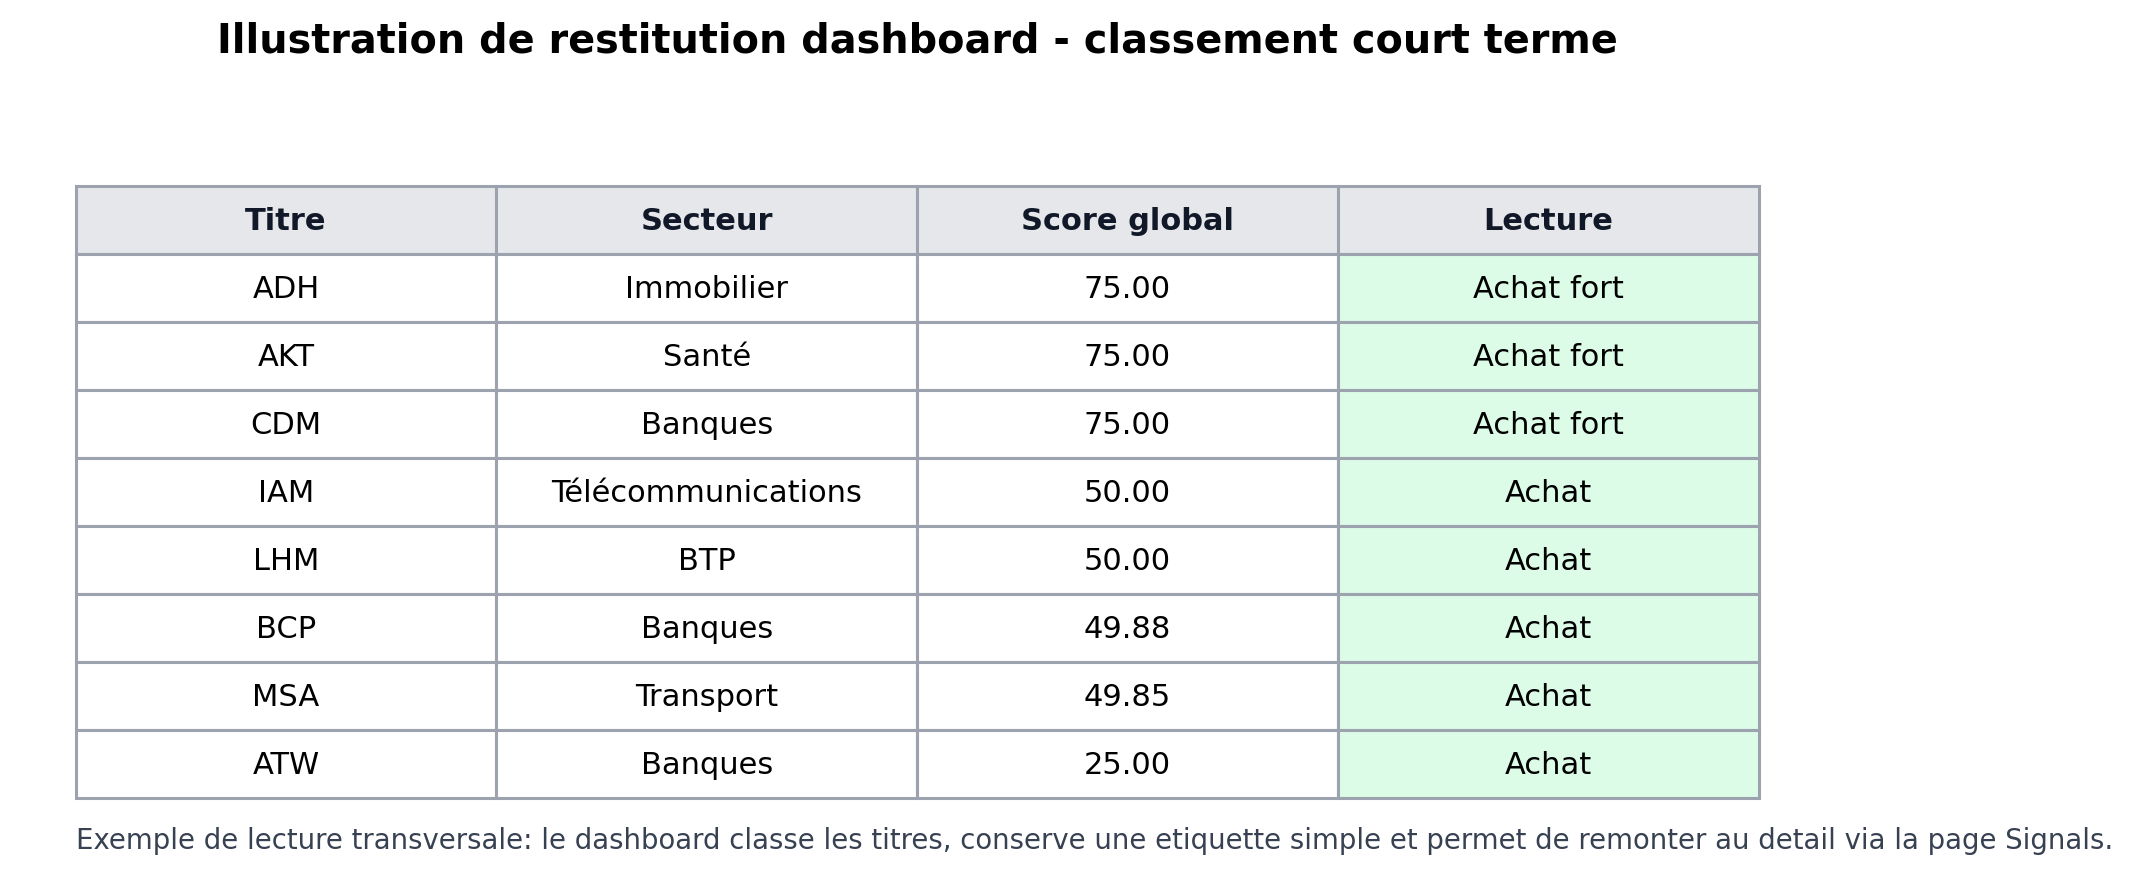
\includegraphics[width=\textwidth]{figures/desk_signal_report/dashboard_ranking.png}
\caption{Illustration de restitution dashboard à court terme.}
\end{figure}

La vue dashboard transforme le moteur en outil de priorisation. À court terme, plusieurs titres ressortent immédiatement, tandis que d'autres appellent une lecture plus prudente. Ce mode de restitution aide le desk à passer plus vite de l'univers couvert à une short-list de cas à regarder.

\begin{figure}[H]
\centering
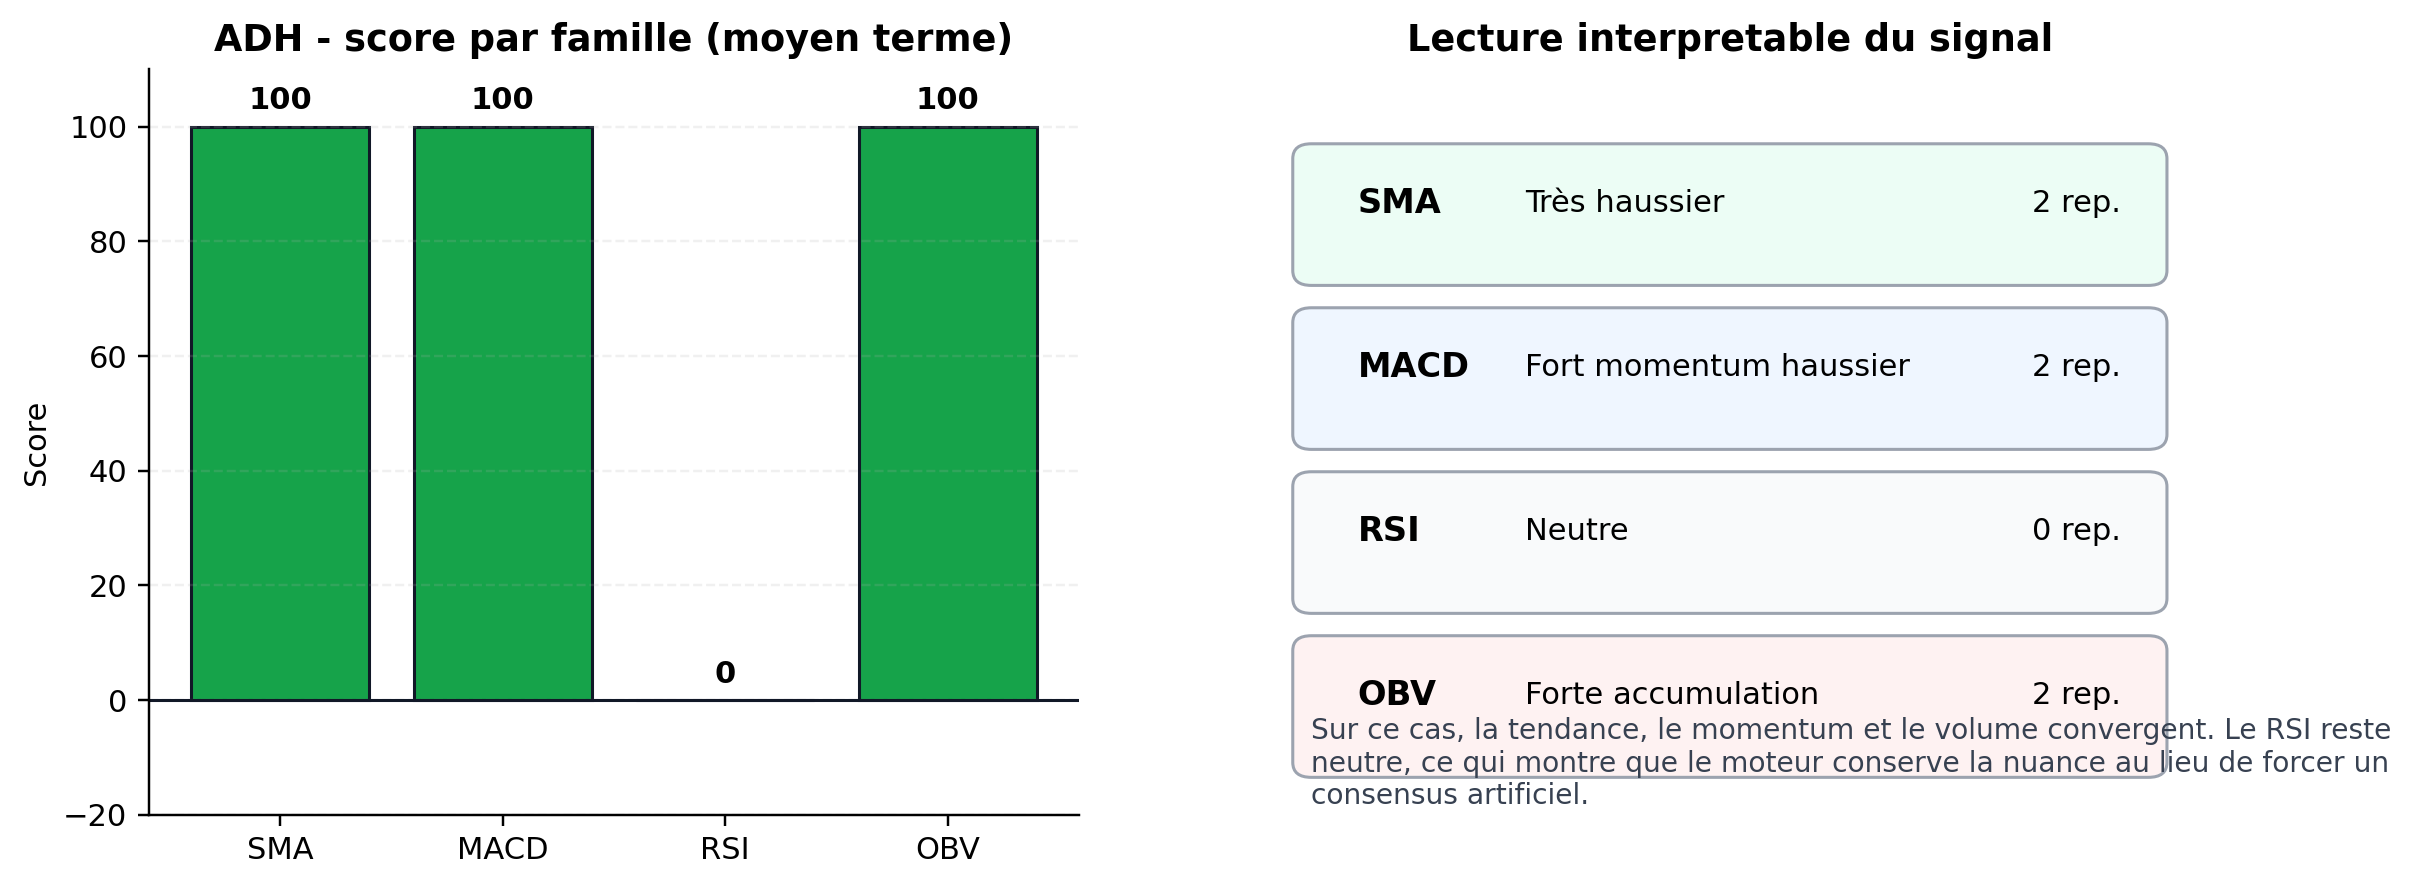
\includegraphics[width=\textwidth]{figures/desk_signal_report/adh_breakdown.png}
\caption{Exemple de lecture détaillée : ADH en horizon moyen terme.}
\end{figure}

Le cas \textbf{ADH} est parlant. En moyen terme, le titre ressort en \textbf{Achat fort} avec un score global de \textbf{+75,0}. La tendance, le momentum et le volume convergent, tandis que le RSI reste neutre. Cette nuance est importante : le moteur ne cherche pas à rendre toutes les familles artificiellement positives. Il conserve l'information utile, même lorsqu'elle n'est pas parfaitement uniforme.

\section*{5. Valeur ajoutée pour le desk}

Le produit apporte une valeur métier sur cinq plans.

\begin{itemize}
\item \textbf{Homogénéité de lecture} : la même logique est appliquée à l'ensemble des titres.
\item \textbf{Priorisation} : le dashboard permet de passer d'une lecture dispersée à une lecture ordonnée.
\item \textbf{Explicabilité} : il est possible de remonter du score global aux familles, puis aux représentants retenus.
\item \textbf{Lecture multi-horizon} : le desk peut distinguer un signal tactique d'une lecture plus structurelle.
\item \textbf{Discipline méthodologique} : le recours à l'évaluation \textit{out-of-sample} limite les lectures trop opportunistes.
\end{itemize}

En pratique, le produit ne remplace pas la décision humaine. Il améliore la qualité du point de départ analytique : mieux voir, mieux comparer, mieux justifier.

\section*{6. Limites et perspectives}

Le produit reste volontairement sobre dans son périmètre actuel.

\begin{itemize}
\item Le cœur publié et présenté repose sur \textbf{quatre familles} ; cela favorise la lisibilité, mais ne couvre pas encore tout le spectre de la lecture technique.
\item La qualité du signal dépend directement de la qualité et de la fraîcheur des données de marché.
\item Le produit doit être lu comme un \textbf{outil d'aide à l'analyse}, et non comme une consigne d'exécution.
\end{itemize}

Les perspectives les plus naturelles sont déjà identifiées :

\begin{itemize}
\item extension progressive du nombre de familles d'indicateurs ;
\item enrichissement de la page Signals et des vues d'exploration ;
\item approfondissement de certaines couches de lecture déjà amorcées ;
\item renforcement de la restitution comparative entre titres, secteurs et horizons.
\end{itemize}

\vspace{0.6em}
\fcolorbox{black}{gray!8}{%
\parbox{0.96\textwidth}{%
\textbf{Conclusion.} Le produit présenté constitue une brique crédible pour un environnement de desk actions : le moteur de signaux apporte la rigueur, la page Signals apporte l'explication, et le dashboard apporte la synthèse. L'ensemble ne remplace pas le jugement du desk ; il lui donne un cadre de lecture plus robuste et plus exploitable.
}}

\end{document}
